\chapter{The Network Machine Learning Landscape}
\label{sec:ch1}

In this section, we'll cover the basics of the network machine learning landscape. We learn a lot of high level elements about networks, and introduce some of the basic terminology for network data. This will give you an understanding of the basics of the network data structure, which will make Chapter \ref{sec:ch4} more digestible when we formally introduce network data structures and how you can manipulate them. 

We take a look at the different types of problems you might come across in network machine learning, and how network data fits into the types of problems you want to adress. Then, we'll see how a particular branch of mathematics,  \emph{statistics}, fits into the machine learning landscape. This chapter will be very high level, but will allow you to see how the pieces of the book fit together in the grand scheme of things. 

Here are some basic questions that we will approach in these next sections:
\begin{enumerate}
    \item How do networks fit into the world of machine learning, and why are they important?
    \item What does it mean to learn from a network, and what kinds of things would you be trying to learn?
    \item How can we use network-valued data to understand the world better?
\end{enumerate}

Having a good understanding of the high level will help you see how the lower level parts fit together in terms of your ultimate goal of applying network machine learning to new and exciting problems in your work. 

\newpage 

\section{What is network machine learning?}
\label{sec:ch1:whatis}

If you are reading this book, you probably have some idea what the term ``machine learning'' means. According to wikipedia \cite{wikiML}, machine learning is a field of inquiry devoted to understanding and building methods that {learn}; that is, methods that leverage data to improve performance on some set of tasks.

For instance, if you have an image and you are a photo editor working in pattern recognition, you might want to learn how you can automatically segment a person so that you can blur the background, (see Figure \ref{fig:ch1:ml-ex}. ) If you are doing natural language processing, you might want to learn how identify the unique instruments in the song on an audio track. If you are a scientist, you might want to learn how a lobster's size correlates with its age so that you can predict lobsters' average age.  What unites these examples is that in all of them you are using data,  to learn something so that you can accomplish some task. Machine learning has grown enormously over the past few decades, and the use-cases of machine learning are rapidly coming to pervade modern life.

\begin{figure}[h]
    \centering
    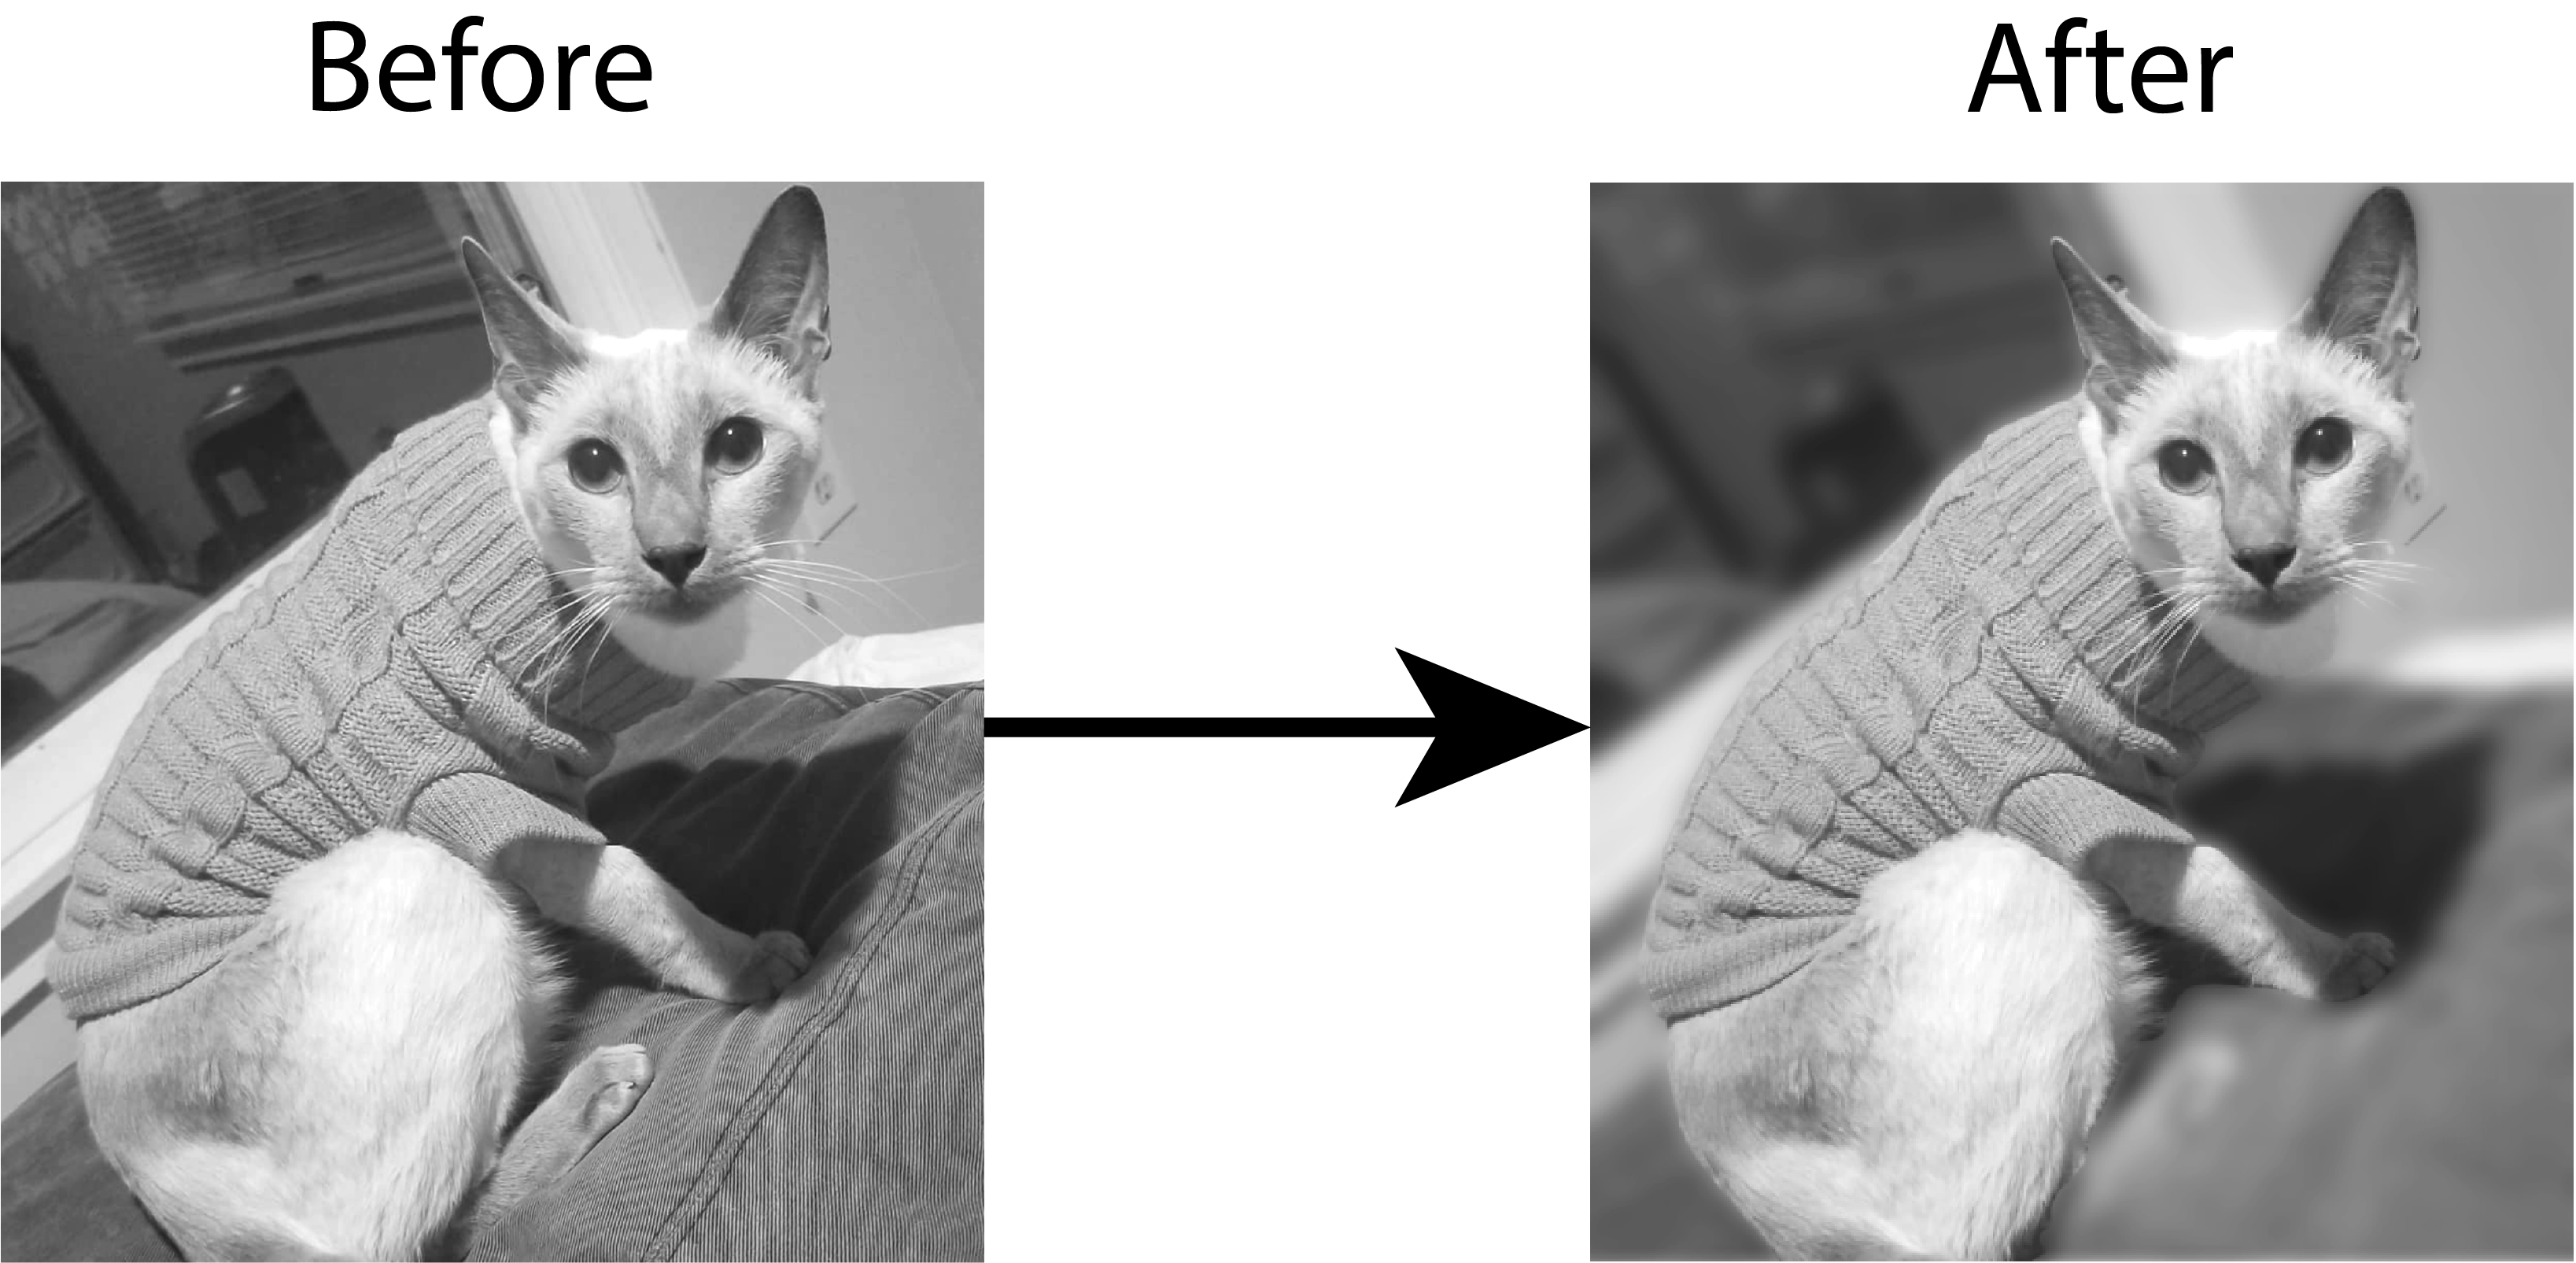
\includegraphics[width=\linewidth]{foundations/ch1/Images/cboy.png}
    \caption[Machine learning task]{Learning how to segment an image to blur the background. A machine learning system is trained using numerous images with the foreground segmented out. This trained system is then used to segment out the foreground on new images, and then the background is blurred.}
    \label{fig:ch1:ml-ex}
\end{figure}


\subsection{Traditional machine learning leverages tabular data structures}

In traditional machine learning, data follows what is called a \textit{tabular} format. This means that the data are arranged in a table or an array, where each row represents a single observation. We recommend you check out the Pandas tutorial on tabular data \cite{pandastut}. 

Conveniently, a lot of modern developments in machine learning apply directly to tabular data. This means that, with some amount of effort, one can take techniques developed in one domain of machine learning, and readily modify or apply them to problems in another domain of machine learning, without needing to {reinvent the wheel}. By this we mean that you can focus your effort on your problem, and borrow techniques developed for related problems, without having to start from scratch every time. For example, if you had a tabular dataset where each row represented a lobster with two columns representing the length and sex of the lobster, you might try to learn how these columns can be used to predict the lobster's claw size. You could do this using an extremely general approach, by simply producing a line of best fit for the claw size depending on which biological sex a lobster is. 

In Figure \ref{fig:ch1:tabular-dat}, we look at how tabular data fits into a machine learning system. This example comprises a basic classification task, in which each observation is either blue or orange. Some of the data (the {training set}, circles) is used to train a machine learning algorithm ({learning}, the transparent blue and orange voronoi cells), and the remainder of the data is used to test the trained algorithm on new data ({evaluating} on the squares using the voronoi cells learned). The trained model can then be further refined ({updated}), or deployed for your intended use-case.

\begin{figure}[h]
    \centering
    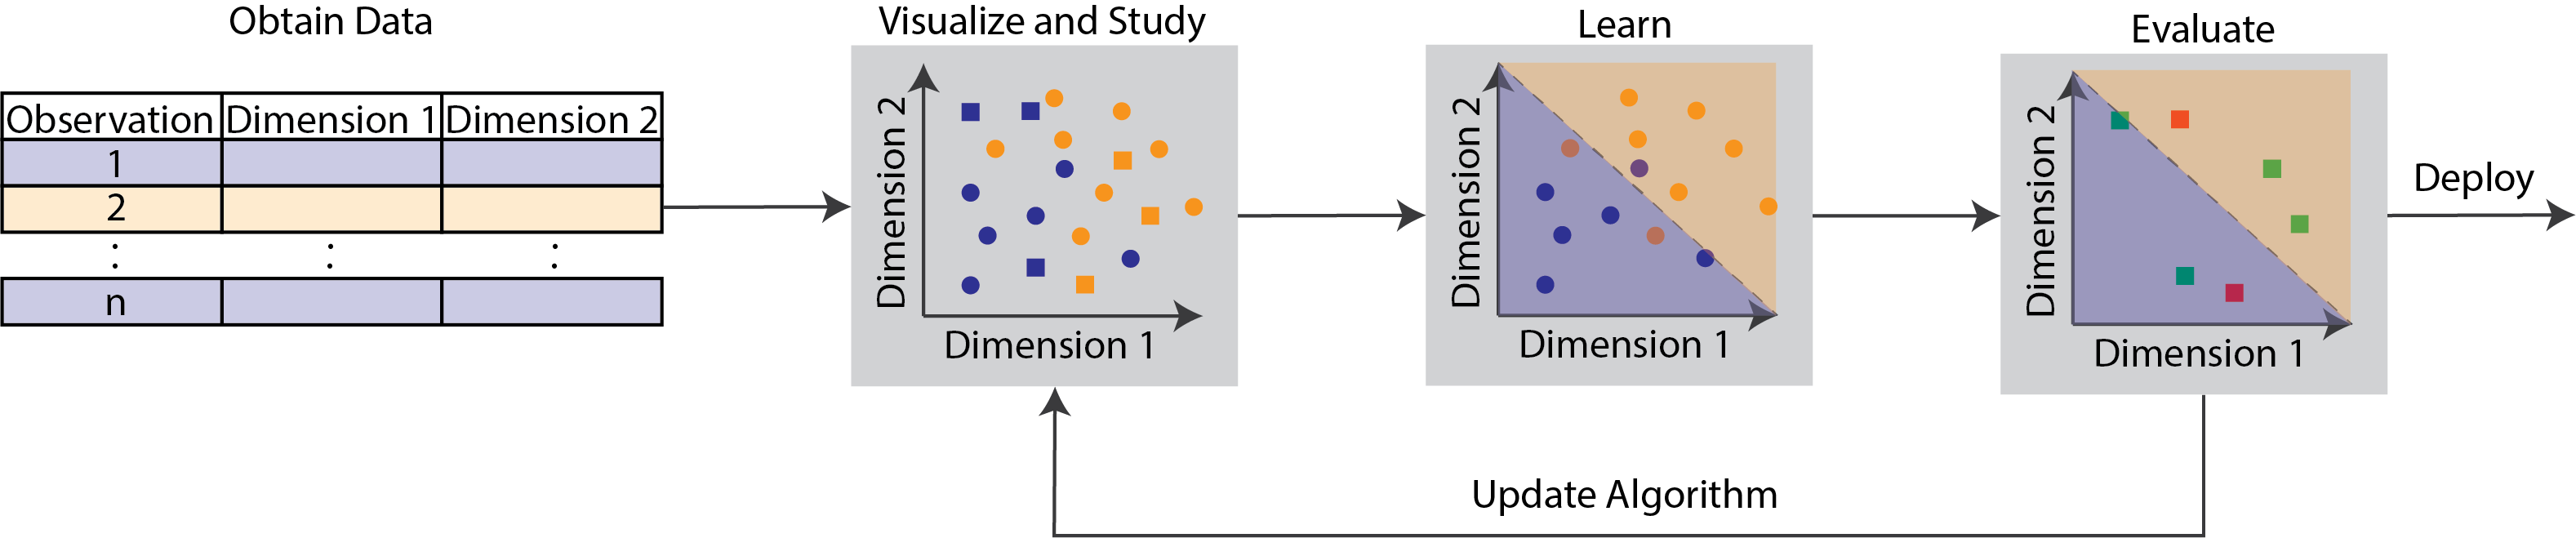
\includegraphics[width=\linewidth]{foundations/ch1/Images/ml_ex.png}
    \caption[Machine learning system]{Machine learning systems start by obtaining inputs as tabular data, where the rows are observations and the columns are features, i.e.  \textit{dimensions} of each observation.}
    \label{fig:ch1:tabular-dat}
\end{figure}

\subsection{What is a network?}

So, what does this have to do with networks? As it turns out, in the 21st century, networks are all around us. When most people think of a ``network'', they often have some vague image in their head of the internet, or of cell phone towers transmitting data, or of some other technical system. But networks have a specific definition in the world of machine learning and data science. The most direct example can easily be explained through the recent rise in social media over the last decade. In a network, your data follows a prescribed pattern: a group of items (say, people on the social network) are interconnected to one another through clearly defined relationships (say which people are friends with one another in the network). 

In other places, you might hear networks referred to as ``graphs'', and the field studying them as ``graph theory''. We try to avoid this terminology in this book, since it's easy to confuse a graph and a plot with an $x$/$y$ coordinate axis. We'll stick to the term ``network'' throughout this book when possible. There might be times when we choose to use the word ``graph'', since the name of some algorithm or tool we're showing you uses it, but just remember that they mean the same thing.

\begin{figure}[h]
    \centering
    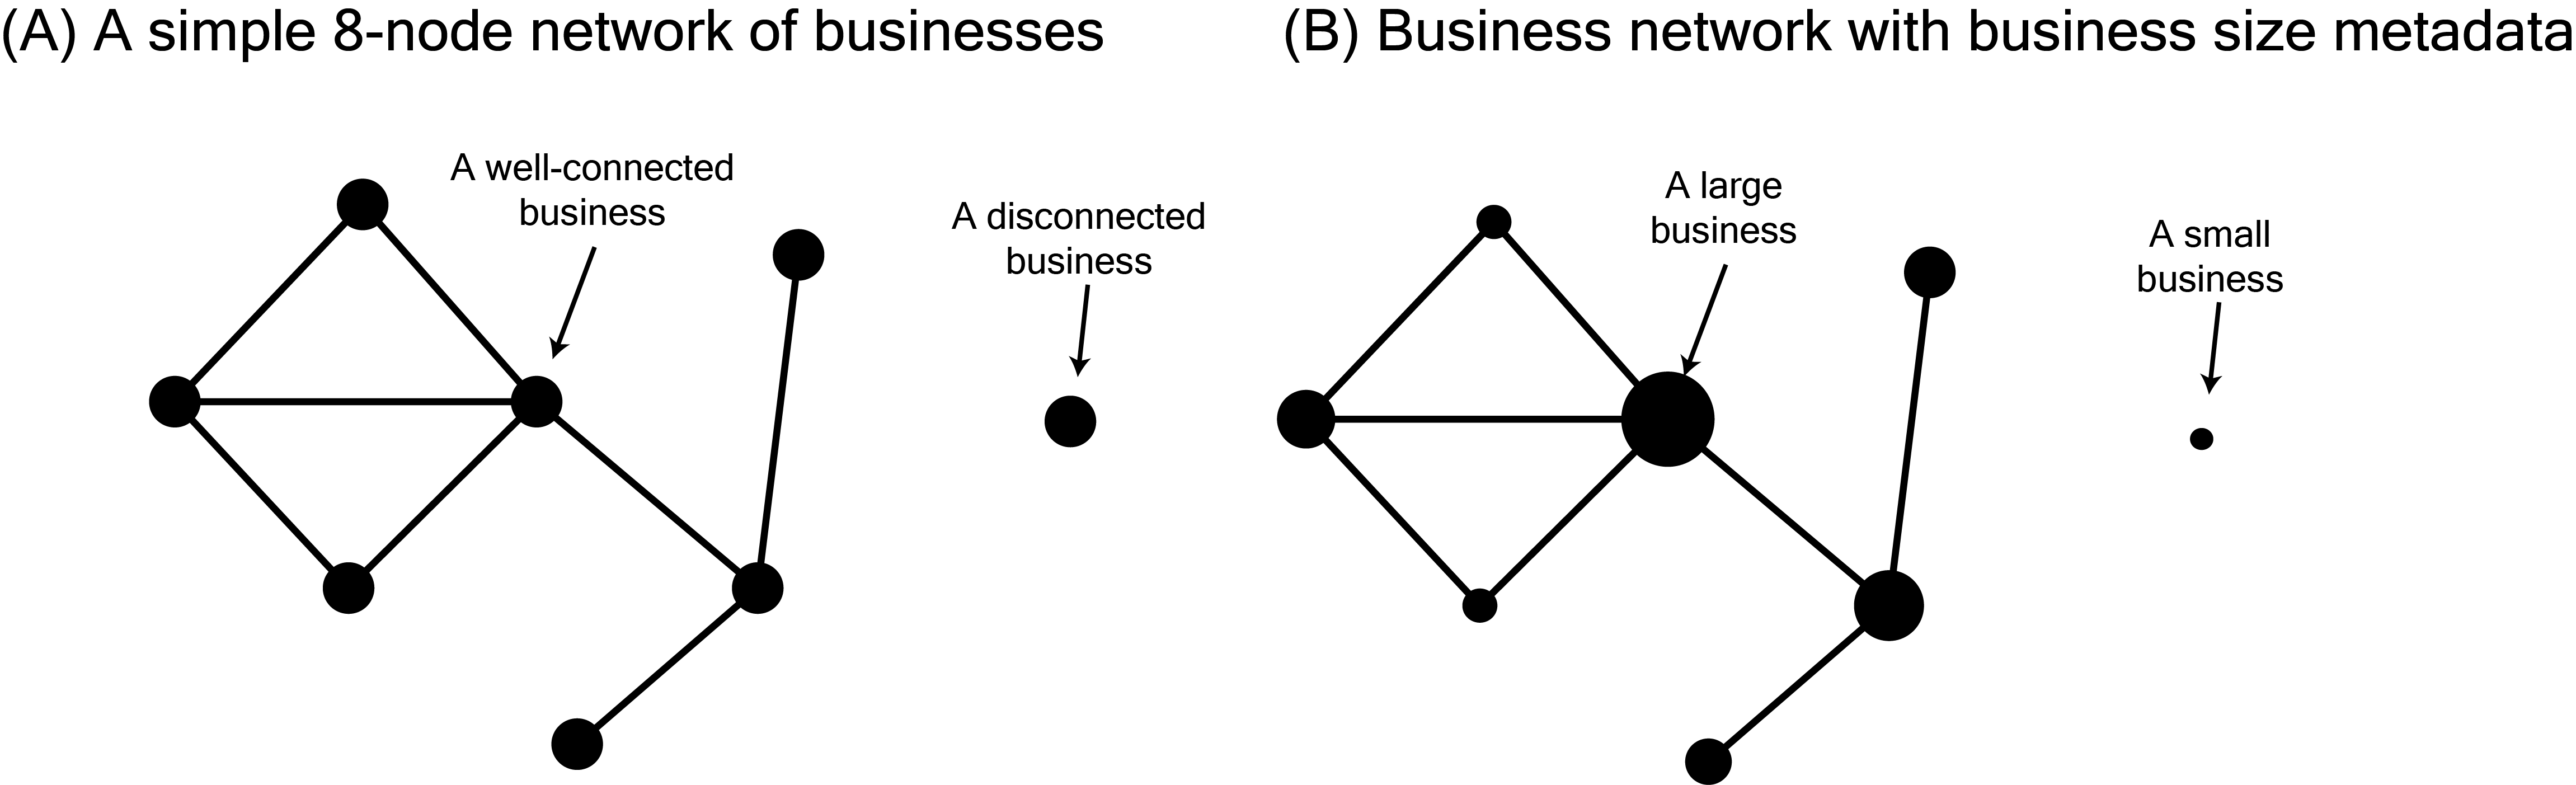
\includegraphics[width=\linewidth]{foundations/ch1/Images/simp_net.png}
    \caption[Simple network example]{\textbf{(A)} indicates a simple network, where nodes are businesses, and edges exist if a given pair of businesses transact with one another. \textbf{(B)} indicates the same simple network, but each node also has a piece of information attached to it, the number of employees (indicated by the node size).}
    \label{fig:ch1:simplenet}
\end{figure}

Let's get more specific about what we mean. Each object in your network is called a \textit{node}, or a vertex (for consistency we'll stick to "node" in this book). A connection between two nodes is called an \textit{edge}. Below you can see a visualization of a simple network with 8 nodes. As you can see, some nodes are well-connected with other nodes -- for example, the node in the center, has edges to five other nodes -- and you can also have nodes which aren't connected to anything, like the lonely extra node without any edges. This is illustrated in Figure \ref{fig:ch1:simplenet}(A).

Networks might also contain extra information. Each node might have a set of features attached to it: extra information that comes in the form of a table. Say the network we just made represents business transactions. Assume that there are eight companies, one corresponding to each node, and there is an edge if one company has sold something to another.

Then, we might also have information about the company size. If the company is larger, you might assume that it'll tend to have had more business transactions with the other companies. The network, in this case, includes the company size information. This is illustrated in Figure \ref{fig:ch1:simplenet}(B).

\subsection{Why do we study networks?}
\label{sec:ch1:howstudy}

If you think about it, you can see networks everywhere. The objects could be people, and the edges could be friendships. Or the objects could be computers, and the relationship could be the information they send to each other. if you're working in air traffic control, you'd have flight networks where the edges are flights from City A to City B; or if you're an epidemiologist studying disease, you could create an infection network. Neuroscientists explore brain networks, consisting of neurons and their relationships with each other, and computer scientists often use neural networks, which have become pillars of machine learning.

Networks can even be used to visualize ideas: in a Bayesian network, nodes represent a set of variables and the edges represent their conditional dependencies. In a correlation network, nodes represent variables, and the edges represent the correlation between those variables. You can have ecological networks, electrical networks, gene networks, or you could visualize your team's workflow with a network.

Even the way we think can be thought of as a network. Visualize a concept or object in your head. Maybe you could think about the food you had for breakfast this morning, or the city you live in. Now, think about the connections between those concepts and others. Maybe you had eggs and toast for breakfast. Eggs and toast are connected with a multitude of other concepts in your head: forks and silverware, kitchens, hunger, protein, carbohydrates, your morning routine, chickens, wheat, other breakfast foods, and innumerable other things. What you're doing right now is exploring a small part of the massive semantic network that exists in your head.

Network machine learning is a relatively new field. The vast majority of it has been invented (or discovered) after the year 2000, and many fundamental proofs have only been published recently. 

For the business-minded readers out there, this is an incredible time to learn about networks. Graph neural networks (GNNs) are becoming increasingly popular as deep learning and neural networks proliferate. This book provides the basic foundational concepts and intuition required to understand how, when, and why GNNs, or any other network machine learning tool, work.

Real-life applications also follow a general trend. It begins with academics spending a lot of time, usually 10-20 years, publishing proof-of-concept papers, discussing possible approaches to solve problems, and developing fundamental tools (usually informally, with somewhat messy code that exists in jupyter notebooks). Then, as the field of research starts maturing, companies and industry people start noticing these new academic tools. They find ways to apply them to make their product or service better, and they develop easy-to-use packages like \texttt{scikit-learn} to make these academic tools mainstream. Network machine learning is at a tipping point right now: its academic foundations have been built up over the past 10-20 years, and the tools for building and working with networks are now starting to move from academia to industry. Congratulations: you could get in early for a wave of application-focused network machine learning tools!


\subsubsection{Why do we need special machine learning approaches for networks?}

As you will learn throughout this book, the problem you run into is that networks mostly exist not in their most naive form, tabular data, but instead in network-valued data. This means, unfortunately, that all those techniques that were developed over decades for tabular data cannot, natively, be used for network-valued data. However, as we will see, we can take various approaches to {adapt} networks to a more traditional format, including tabular structures using network representations. Once we adapt these networks  to more traditional structures, we can then apply techniques from other domains of machine learning to learn about our networks. In Figure \ref{fig:ch1:nml-high-level}, we see how network machine learning functions at a high level. Loosely, \textit{network machine learning} is machine learning for network-valued data (data which is a {network}, not a {tabular structure}). 

\begin{figure}
    \centering
    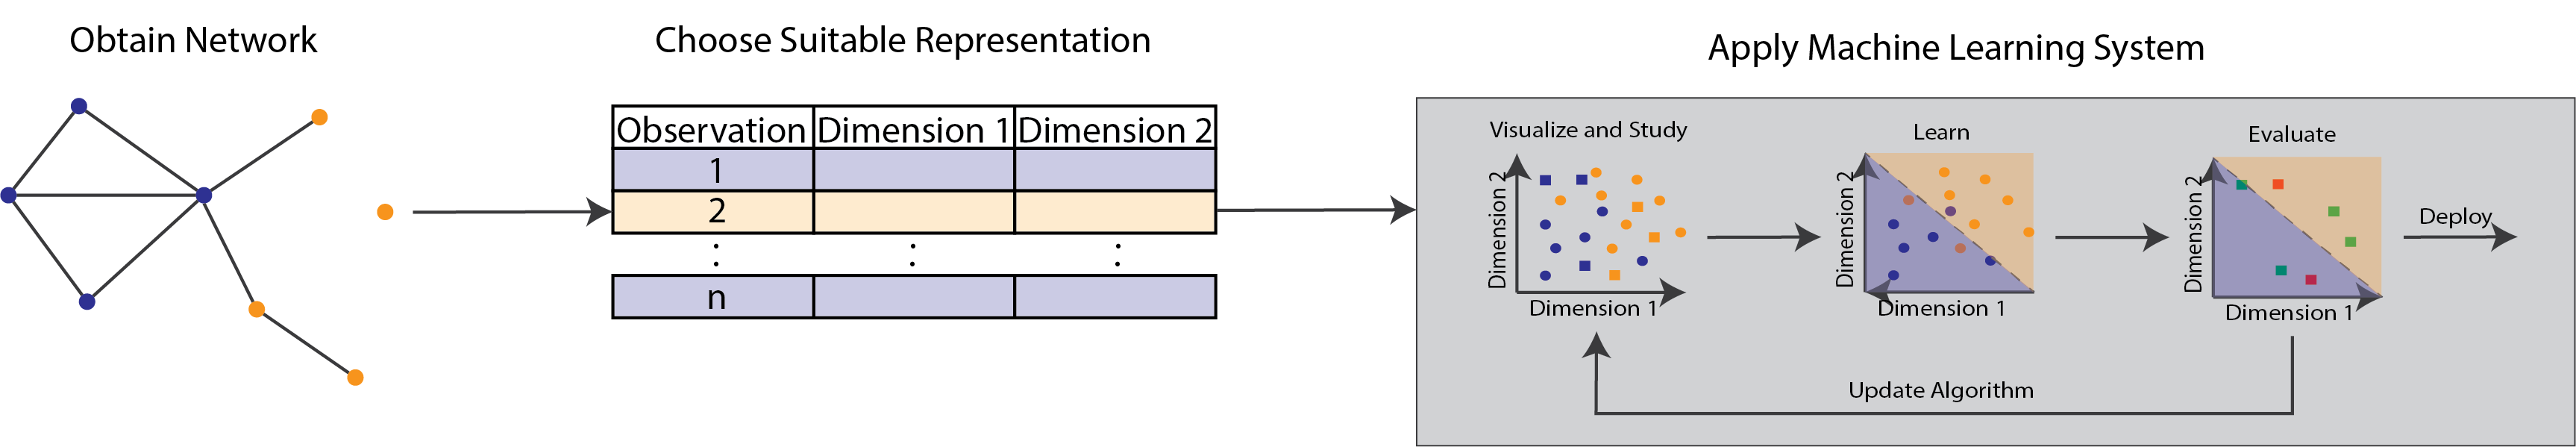
\includegraphics[width=\linewidth]{foundations/ch1/Images/nml-high-level.png}
    \caption[Network machine learning]{In network machine learning, we start by obtaining a network. The first step in network machine learning is to select a suitable representation for the network, which depends on the type of questions you are asking. Using this representation, you apply a machine learning system which is suited appropriately for the type of task that you have. As the set of questions one might have about network data may differ from a typical tabular dataset, the manner in which these techniques are applied may need to be tuned for the question of interest.}
    \label{fig:ch1:nml-high-level}
\end{figure}



Let's get started!

\newpage
% \section{Why do we study networks?}
\label{sec:ch1:howstudy}

When you start thinking, you start seeing networks everywhere. The objects could be people, and the edges could be friendships. Or they could be computers, and the relationship could be the information they send to each other. You'd have airflight networks if you're working in air traffic control, where the edges are flights from city A to B; or if you're an epidemiologist studying disease, you could create an infection network. Neuroscientists can explore brain networks, which tell them about neurons and their relationships with each other, and computer scientists often use neural networks, which have become pillars in machine learning.

Networks can even be used to visualize ideas: in a Bayesian network, your nodes represent a set of variables and the relationship between them is their conditional dependencies. In a correlation network, your nodes represent variables, and the edges represent the correlation between those variables. You can have ecological networks, electrical networks, gene networks, and you could visualize your team's workflow with a network.

Even the way we think can be thought of as a network. Visualize a concept or object in your head. Maybe you could think about the food you had for breakfast this morning, or the city you live in. Now, think about the connections between those concepts and others. Maybe you had eggs and toast for breakfast. Eggs and toast are connected with a multitude of other concepts in your head: forks and silverware, kitchens, hunger, protein, carbohydrates, your morning routine, chickens, wheat, other breakfast foods, and an innumerable amount of other things. What you're doing right now is exploring a small part of the massive semantic network that lives in your head.

Network machine learning is a relatively new field. The vast majority of it has been invented (or discovered) after the year 2000, and many fundamental proofs have only been published recently. 

For the business-minded folks out there, this is an incredible time to learn about networks. Graph neural networks (GNNs) are becoming increasingly popular as deep learning and neural networks explode. This book provides the basic foundational concepts and intuition required to understand how, when, and why GNNs, or any other network machine learning tool, work.

Real-life applications also follow a general trend. You'll see academia spend a lot of time, usually 10-20 years, publishing proof-of-concept papers, discussing possible approaches to solve problems, and developing fundamental tools (usually informally, with somewhat messy code that exists in jupyter notebooks). Then, as the field of research starts maturing, companies and industry people start noticing these new academic tools. They find ways to apply them to make their product or service better, and easy-to-use packages like scikit-learn are developed to make these academic tools mainstream. Network machine learning is at a tipping point right now: its academic foundations have been built up over the past 10-20 years, and the tools for building and working with networks are now starting to move from academia to industry. Congratulations: you could get in early for a wave of application-focused network machine learning tools!

\section{Types of network machine learning problems}
\label{sec:ch1:types}


There are many different types of network machine learning systems. We tend to broadly group them into the following categories:
\begin{itemize}
\item whether or not they involve one or multiple networks (single or multiple network learning systems),
\item whether or not they require additional information in the form of network attributes (attributed or non-attributed network learning systems),
\item whether they ask questions about an edge, a node, a group of edges/nodes, or about the network itself, and
\item whether or not the approach can be used in isolation from a statistical model (non-model based or model-based network learning systems).

\end{itemize}

To learn about these criteria, we'll use a few running examples:

\begin{floatingbox}[h]\caption{Brain networks for musicians and non-musicians}
\label{box:ch1:brainnet}
You have brain networks that were acquired from a large group of people. The nodes of this network represent areas of the brain, and the edges represent whether a pair of brain areas can communicate using neurons. Neurons are cells in the brain that receive sensory input from the environment, and work together to transform the sensory input into usable outputs (thoughts, actions, behaviors, etc.) Each brain network is from a person who we know is either a non-musician or a musician.
\end{floatingbox}

\begin{floatingbox}[h]\caption{A pair of social networks for students at a school}
\label{box:ch1:social}
In this network, the nodes represent students who attend one of two schools. Edges represent whether the students are connected on a social media site. We have networks collected from two social media sites, Facebook and Twitter.
\end{floatingbox}

\subsection{Single vs multiple network learning systems}

\subsubsection{Single network learning systems}

In many cases of network learning, you only actually have a single sample: the network itself. A \textit{single network learning system} is a system in which insight is derived from a single network, that is one collection of nodes and edges. In a single network learning system, you only have one sample: the network itself. In a traditional machine learning framework, having a single sample is disastrous: you canot derive insight with one sample in a traditional machine learning framework, because a question cannot be addressed using only one data point. This is an extreme case of the small sample problem. As an example, if you wanted to determine the degree to which cloud cover predicted whether or not it was raining, and you only had one day's worth of data, you would not be able to learn anything, because your answer would totally be determined by whether or not it was cloudy on that particular day and whether or not it was raining on that particular day.

On the other hand, in network learning, a single sample is far from disastrous. While we only have one network, that one network is defined by a collection of nodes and edges. For this to be meaningful, there must be multiple nodes and edges in the first place! While you might only have one network, you can still learn about relationships that exist among the nodes, edges, or both. The caveat is that the conclusions you reach from your network might be limited to the specific network you are studying, or a rather limited sample population, but often that’s not much of a problem.


Most of the strategies in this book address single network learning systems.


\subsubsection{Multiple network learning systems}

A \textit{multiple network learning system} is a system in which insight is derived from multiple networks, wherein you have multiple collections of nodes and edges. Unlike a single network learning system in which you can only obtain conclusions on the basis of characteristics of that particular network itself, in a multiple network learning system, you can obtain insights {both} within and across the networks.


In the brain networks from Example \ref{box:ch1:brainnet}, you can derive insights to describe the commonalities among the brain networks of non-musicians along with the commonalities among the brains of musicians, and then compare them to look for differences between the brain networks of non-musicians and musicians.


Some strategies which employ multiple network learning systems are:
\begin{itemize}
\item multiple network representation learning in Section \ref{sec:ch6:multinet},
\item anomaly detection in Section \ref{sec:ch9:anomaly}, and
\item signal subnetworks in Section \ref{sec:ch9:ssn_incoherent}.
\end{itemize}

Note that these these categories are not mutually exclusive, and a network machine learning system will pull elements from several of the different categories simultaneously. For instance, you might have a machine learning system that is a single network, node-attributed, non-model-based machine learning system like a community detection algorithm.

\subsection{Non-attributed vs richly-attributed network learning systems}

In machine learning, you are probably familiar with the terms unsupervised and supervised learning. In network learning, we tend to use a more specific name for these two ideas.


\subsubsection{Non-attributed network learning systems}

The concept of a non-attributed network learning system is directly analogous to the concept of fully unsupervised machine learning. \textit{Unsupervised learning} can be loosely defined as a learning problem in which the data you feed to the algorithm does not include the desired solutions, called \textit{labels}. We call a network learning system \textit{non-attributed} if at the time of analysis, the network(s) you feed your algorithm includes only nodes and edges.


For instance, let's consider the Facebook network from Example \ref{box:ch1:social}. Suppose, unfortunately, that you've lost the information about which students attend which school. You hypothesize that there might be two groups of students in the network, called {communities}, and that if a student is in particular community, they tend to be better friends with other students in the same community. You want to see if you can identify these communities programmatically, and perhaps recover the school information for each student. A non-attributed network learning problem is shown in Figure \ref{fig:ch1:nonattr}. Perhaps, the groups of nodes that are heavily connected (indicated by the gray circles) corresponds to the schools that each student attends.

\begin{figure}[h]
\centering
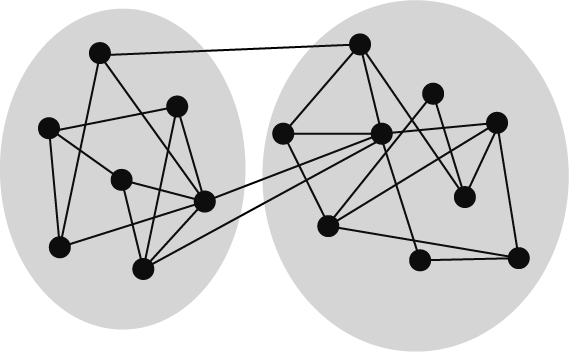
\includegraphics[width=0.5\linewidth]{foundations/ch1/Images/nonattr_ex.png}
\caption[School network hypothesis]{A school network, where the nodes are students and the edges indicate which pairs of students are friends.}
\label{fig:ch1:nonattr}
\end{figure}


Some examples of non-attributed network learning systems are:
\begin{itemize}
\item network embeddings in Section \ref{sec:ch6},
\item community detection in Section \ref{sec:ch7:comm_detect},
\item latent position comparisons in Section \ref{sec:ch8:twosample}, and
\item anomaly detection in Section \ref{sec:ch9:anomaly}.
\end{itemize}


\subsubsection{Attributed network learning systems}

Similarly, the concept of an attributed network learning system is analogous to the concept of supervised or semi-supervised machine learning. \textit{Supervised learning} can be loosely defined as a learning problem in which the data you feed to the algorithm includes {labels}, and \textit{semi-supervised learning} can be loosely defined as a learning problem in which the data you feed to the algorithm includes \textit{some} of the labels. A network is an \textit{attributed network learning system} if at the time of analysis, the network(s) you feed your algorithm include attributes in {addition} to nodes and edges. We have four main types of attributed network learning systems. They are:
\begin{itemize}
\item Networks with node attributes,
\item Networks with edge attributes,
\item Networks with network attributes, and
\item Networks with multiple-network attributes.
\end{itemize}


\paragraph{Networks with node attributes}

A network with \textit{node attributes} is a collection of nodes and edges where, for each node, you have an additional piece of information to describe that node. Let’s consider the school example we talked about above in the section on non-attributed network learning systems. For each student, you also have an additional piece of information: you know which school each student attends, and you want to investigate whether the probability of two students being friends is higher in school one or in school two. A problem for networks with node attributes is shown in Figure \ref{fig:ch1:netnode_edge_attr}(A). 

\begin{figure}[h]
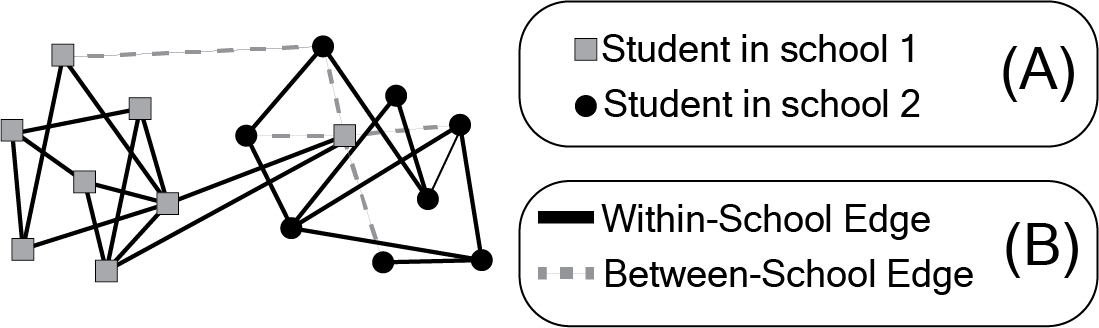
\includegraphics[width=\linewidth]{foundations/ch1/Images/nodeedge_attr.png}
\caption[School with node and edge attributes]{\textbf{(A)} the school network for Facebook, approached using node attributes. \textbf{(B)} the school network for Facebook, approached using edge attributes. Instead of focusing on the school assignments of the nodes, we focus on two groups of edges (the within-school edges, and the between-school edges).}
\label{fig:ch1:netnode_edge_attr}
\end{figure}


Some examples of problems which deal with node attributes are:
\begin{itemize}
\item 

joint representation learning in Section \ref{sec:ch6:joint},

\item 

model selection in Section \ref{sec:ch7:modelselect},

\item 

testing for differences in block matrices in Section \ref{sec:ch8:twosamplesbm}, and

\item 

testing for differences between groups of edges in Section \ref{sec:ch7:testing}.

\end{itemize}

\paragraph{Networks with edge attributes}

A network with edge attributes is a network consisting of nodes and edges where, for each edge, you have an additional piece of information to characterize that edge. For instance, if we return to the Facebook school network from Example \ref{box:ch1:social} that we posed above, we could entirely ignore the school assignments, and simply focus on whether the students have more friends within schools (solid edges) or between schools (dashed edges). This example is shown in Figure \ref{fig:ch1:netnode_edge_attr}(B).


A problem with edge attributes is testing for differences between groups of edges in Section \ref{sec:ch7:testing}.


\paragraph{Networks with network attributes}

A network with network attributes is a collection of networks (each of which has nodes and edges) where, for each network, you have an additional piece of information to characterize that network. Returning to Example \ref{box:ch1:brainnet}, each brain network was from either a musician or a non-musician. This piece of information characterizes each of the networks as either from a musician or a non-musician individual, and applies to the {entire} collection of nodes and edges for a given network. A network with network attributes is shown in Figure \ref{fig:ch1:netnetattr}.

\begin{figure}[h]
\centering
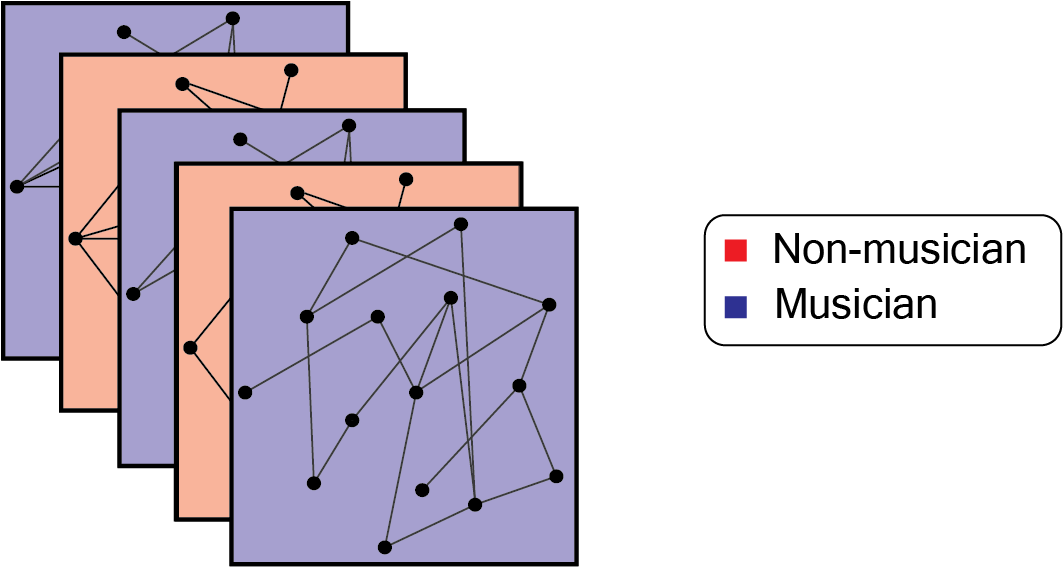
\includegraphics[width=0.8\linewidth]{foundations/ch1/Images/netattr_ex.png}
\caption[Brain networks]{A collection of brain networks, where the nodes are areas of the brain and the edges indicate which brain areas can communicate. For each network, you know whether it comes from a musician or a non-musician.}
\label{fig:ch1:netnetattr}
\end{figure}


An example of a problem which leverages network attributes are signal subgraphs in Section \ref{sec:ch9:ssn_incoherent}.


\paragraph{Networks with multiple-network attributes}

A network with \textit{multiple-network attributes} is a collection of networks (each of which has nodes and edges) where you have additional information that describes how the nodes (or the edges) of the networks relate to one another. Returning to Example \ref{box:ch1:social}, let's add another dimension. The accounts are, for all intents and purposes, anonymous, in that people choose not to share identifying information about themselves on the accounts. However, for three of the people, you know that their two accounts are {matched} together. You want to see if you can use this cross-network attribute (the {matched accounts}) to discover suitable matchings for the remaining accounts in the network. A problem with multiple-network attributes is shown in Figure \ref{fig:ch1:netmultiattr}.

\begin{figure}[h]
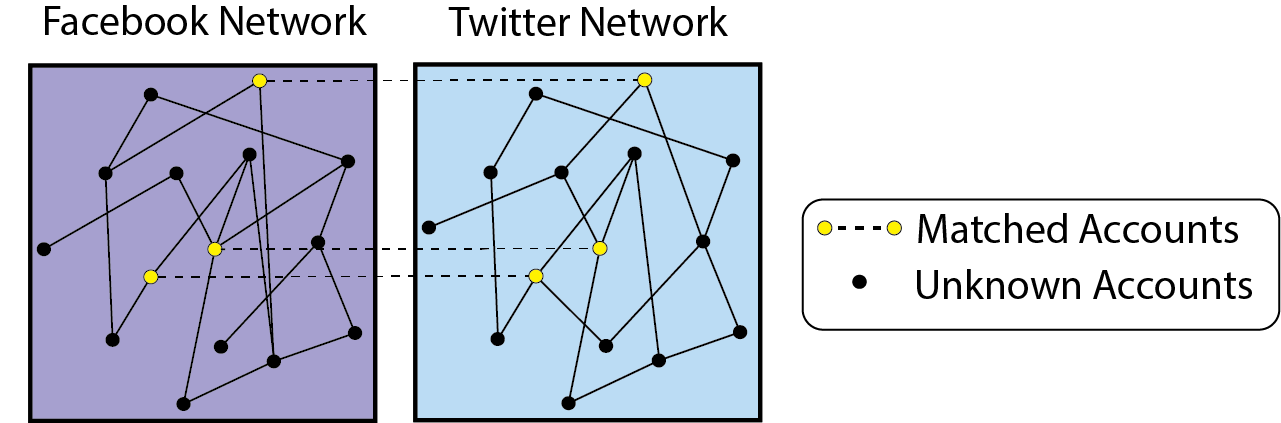
\includegraphics[width=\linewidth]{foundations/ch1/Images/crossnetattr_ex.png}
\caption[Multiple network attributes]{Two social networks from different social media sites. The nodes are people’s accounts on the social media sites (they are the same for both sites) and the edges indicate which pairs of accounts follow one another for that particular site. For three of the people in the network, you know their accounts.}
\label{fig:ch1:netmultiattr}
\end{figure}


An example of problems which leverage cross-network attributes include:
\begin{itemize}
\item Seeded graph matching in Section \ref{sec:ch8:gm}, and
\item Vertex nomination for two networks in Section \ref{sec:ch8:vnviasgm}.
\end{itemize}

\subsection{What part of the network your question is asking about}

In network machine learning, it’s easy to get lost because you're tempted to explore the entire network, whereas your question might be far more limited. For instance, in a transportation network, you might have a collection of nodes representing stations, and a collection of edges representing the number of riders per train during rush hour. You might have a single network for each week of the entire year. We’ll show an example of each type of question from the perspective of the attributes of these networks. 
\begin{enumerate}
    \item Studying a single edge: You might want to know whether a particular edge between two stations could require an additional train because the route is popular during rush hour, and you might only want to study this particular edge over many networks to get some idea of how many passengers take each train.
    \item Studying a single node: You might want to explore the number of passengers who pass through a particular station when deciding whether to approve or reject the expansion of a particular station to include more platforms.
    \item Studying groups of nodes or edges: You might consider cancelling an entire line and need to consider the ramifications of this decision on other stations (groups of nodes) and numbers of passengers per line (groups of edges).
    \item Studying the entire network: You might need to determine whether more funds need to be allocated to public transportation as a whole, and therefore to study how much transportation via the network saves the city over the course of the year.
\end{enumerate}


\subsection{Model-based vs non-model-based network learning systems}

Statistics tends to form somewhat of a ``core'' to network learning systems. This is because in any network learning problem, there is always room for randomness, whether it comes in the form of the particulars of the network you sampled, the set of networks you acquired, the nature of the data you collected, or many other factors. 

We will provide a more rigorous definition later, but for now, you can understand a \textit{statistical model} to be a conceptual framework of a problem that allows you to explicitly account for variation, randomness, or error in your sample (the data you actually obtain) compared to the entirety of the actual object or set of objects that you are studying (the \textit{population}). This balance between model-based and non-model-based network learning is a core aim of this book, so we do not expect you to be able to conceptualize the difference just yet. For this reason, we will try to explain the difference without talking about networks for now.


\subsubsection{Model-based learning systems}

A \textit{model-based learning system} is a system in which a statistical model is required in order to derive your intended meaning from an analysis.

Imagine that you have two coins, and you flip each of them twenty times. You want to understand whether the probability that the two coins land on heads is the same or different. What this means in statistics is that you want to perform a {hypothesis test}: you want to use the data that you obtained (the outcomes of the twenty coin flips for each of the two coins) to determine whether the coins have the same probability of landing on heads (the first hypothesis) or a different probability of landing on heads (the second hypothesis). The \textit{hypothesis test} is the procedure to determine which of the two hypotheses is better supported by the data. This question cannot really be made sense without using a statistical model, because the term {probability} has a statistical interpretation. If you wanted to answer this question, you would need to describe several factors about your experiment a little further:
\begin{itemize}
\item Can each of the coins {only} land on heads or tails, or is there perhaps some other possible outcome? For instance, is one of the coins one centimeter thick and the other a picometer thick, and therefore, the centimeter thick coin has a nonzero probability of landing on its side?
\item For each coin, is the probability that the coin lands on heads {exactly the same} across each of your twenty coin flips for that particular coin? For example, if you flip the coin differently for the first ten flips than you do on the last ten flips, could this artificially make the coin land on heads more or less frequently?
\item Do the outcomes of the coin flips depend on other coin flips? For instance, if you see two straight tails in one of the coins and say a prayer that you get a heads on the next flip, does this affect the probability that the next flip is a heads?
\item Did you collect enough data to determine whether the coins are different? For instance, many statistical tests (including this one) can be interpreted in a variety of ways. When the sample size is tiny, we need to be careful about the assumptions that we make, because statistical testing approaches that we might use (the chi-squared test, for instance) might only be meaningful when we have a lot of data.
\end{itemize}

In order to make a conclusion based on your hypothesis test, you need to be very specific about the assumptions you make about these details of the your data sample, since if any of your assumptions are false, the answer to your question might have a different interpretation. Therefore, you need to understand the assumptions that you made, so that you can make a {decision} based on the outcome of the hypothesis test that you performed.


\subsubsection{Non-model-based learning systems}

For many questions you might want to ask, you could apply techniques from this book in either a model-based or non-model-based manner and be fine either way. What we mean by this is that a lot of questions might be made {intuitive} using a model, but there is no reason you {need} a model in order to answer these questions. A \textit{non-model-based learning system} is a system in which a statistical model is {not} required in order to derive meaning from an analysis.

To make this type of machine learning system a little more concrete, we’ll break down a traditional non-model-based machine learning system. \textit{Principal components analysis} is a procedure which takes data which is {wide} (it has a lot of features or dimensions, which is extremely problematic for many machine learning approaches) and makes it narrower (it has a manageable number of features or dimensions) so that you can use other strategies downstream which might be{more reasonable}, by which we mean that each observation starts with many features, but after applying \texttt{PCA}, each observation has far fewer features. A visual illustration of \texttt{PCA} is shown in Figure \ref{fig:ch1:pcaex}. In this example, we reduce the data from two dimensions (indicated by the $x$ and $y$ axes) to one dimension along the red axis (the first PC).

There is no reason that this procedure cannot be {executed} knowing nothing else about the data: it is simply an algorithm which produces a desired result (making the data manageable for other machine learning techniques). However, if you were to do this and use the intuition of a statistical model (specifically, that the observations are {normally distributed}), you can understand the principal components to be representations of the data that preserve the most {variation}. You can understand variation in this context to be the direction that the data spreads along the most: in Figure \ref{fig:ch1:pcaex}(A), notice that the black points tend to spread out a lot along the red PC, but not as much along the green PC. The degree of variation preserved by the principal components, if you recall, are indicated by principal component scores. This is often desirable intuition for machine learning because if you wanted to apply say \texttt{K-Means} to cluster your observations, you will need the observations from each class to “look” different -- and “looking different” requires variability.

\begin{figure}[h]
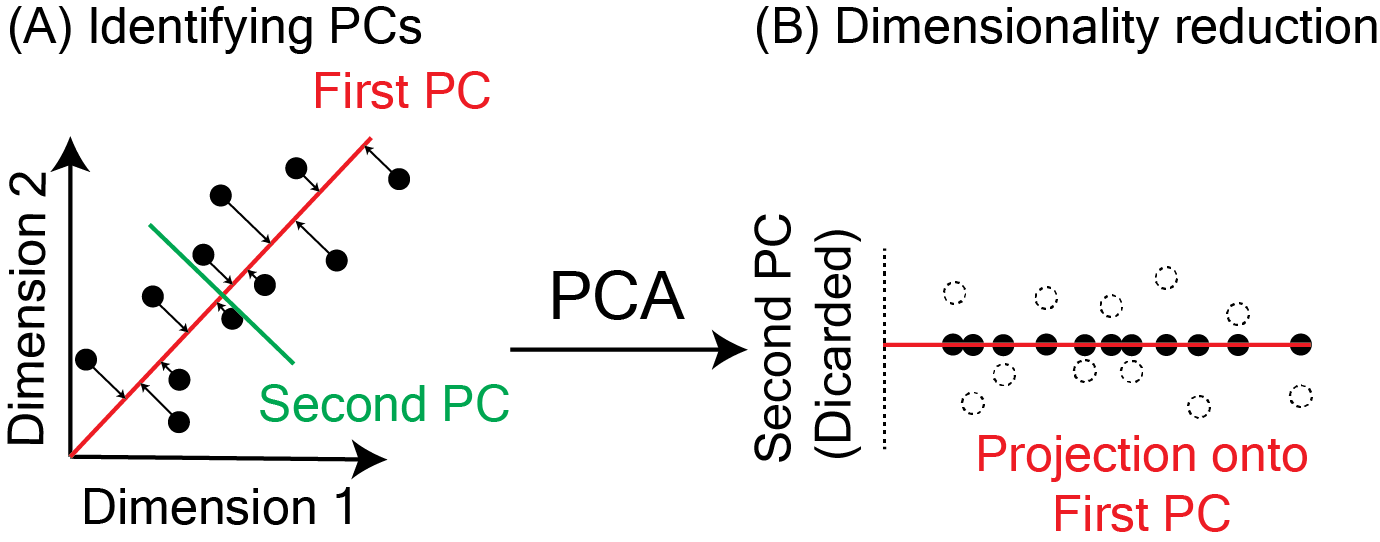
\includegraphics[width=\linewidth]{foundations/ch1/Images/pca_ex.png}
\caption[Principal components analysis]{\textbf{(A)} the observed data shown in the left scatter plot, where the points are two-dimensional. The first ``principal component'' (PC) is the axis in which the data varies the most, and the second PC is the axis (orthogonal to those of the preceding principal components) along which the data varies the second most. Projecting the data to the first PC is shown with the arrows. \textbf{(B)} the data is ``projected'' onto the first PC via PCA, by effectively ``reorienting'' the dataset along the first and second principal components (dashed circles and lines), and then removing the second PC entirely (solid circles) to reduce the dimensionality from two dimensions to one dimension. Think about this in a model-based manner, we ``discarded'' a direction in which the data varies less.}
\label{fig:ch1:pcaex}
\end{figure}

\newpage
\section{Challenges of network machine learning}
\label{sec:ch1:challenges}

Like other branches of science, network machine learning is not without its challenges. There are infinitely many ways in which your network, or networks, that you actually get to analyze might have imperfections which can most efficiently be described as random. Rather than collecting data from every single person on the social network, or obtaining brain networks from every single person who could {potentially} be a musician, or collecting pristine data that always represents the underlying network perfectly, you instead look at a reasonably sized subset of data which you can feasibly obtain. Maybe this means collecting your social network with only $1000$ nodes instead of one hundred million, or maybe this means looking at $200$ brain networks instead of a network from every person in the United States.

In this book on network machine learning, we are going to focus some level of attention on the sub-branch of machine learning known as statistical learning. \textit{Statistical learning} is a framework for machine learning in which we {infer} things about our network by using statistics to refine and conceptualize our problem and quantify how reasonable our conclusions are. What exactly do we mean by this?

\subsubsection{We might imperfectly observe the network}

In many branches of science, collecting network data can be an imperfect and noisy process. It was only recently that we acquired a detailed map of the connectome of a complex organism, the fruit fly larva \cite{Winding2023Mar}. Even though fruit fly larvae are small, this is a substantial undertaking: their brain comprises several thousand neurons, and hundreds of thousands of edges, all fit into a volume smaller than cubic millimeter. In order to study the brain at the neuron-scale, the brain was sliced into thousands of tiny pieces smaller than a human hair, and each piece individually examined with a microscope. From there, extremely complicated algorithms and manual tracing were performed to stitch, slice-by-slice, which neurons connected with which neurons. To make this process even more difficult, everything was done on a single organism; with each step there was extremely minimal room for error. This neuron-by-neuron map was used to construct a network (called the \textit{connectome} of the organism) where the nodes were neurons and the edges were the neuron-to-neuron connections.

\begin{figure}[h]
    \centering
    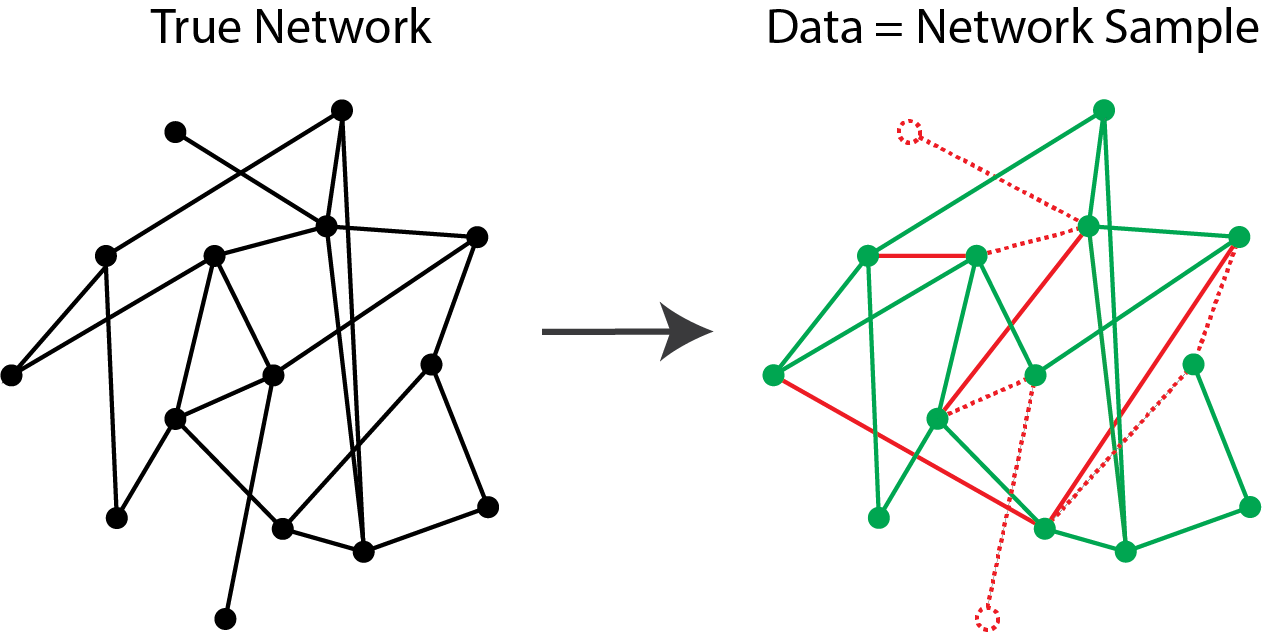
\includegraphics[width=0.7\linewidth]{foundations/ch1/Images/errorful_obs.png}
    \caption[Errorfully observe networks]{The true underlying network contains a lot of information that in the
course of observing or sampling the network, we don't actually measure properly. }
    \label{fig:ch1:errorful_net}
\end{figure}

With so many areas for potential error, it is almost impossible that the network is absolutely perfect. We might have missed some neurons, we might have missed some connections, and there might have been small mistakes anywhere in this complicated process. Figure \ref{fig:ch1:errorful_net} explores what it means for a network to be imperfectly observed. On the left, we see the true network we're trying to obtain. On the right, we see the actual network we obtained: we might be missing some of the nodes (red dashed nodes), we might be missing some of the edges (red dashed edges), or we might see edges which shouldn't really be present (red solid edges). While a portion of the network might faithfully represent the underlying system (green nodes and edges), we don't actually get to see what part of our sample is faithful or unfaithful with respect to the underlying network. The key is that when we attempt to build network machine learning systems, we need to be able to derive insights that are robust to these imperfect observations. This is because in some cases, it might be impossible to ever obtain the data that we need otherwise.

\subsubsection{We might not see the whole network}

When we study a network, it is rare that we observe the entire system perfectly in its entirety. For instance, a social network, in which the nodes of our network are people within the network, and edges are whether groups of people are friends with one another. If we wanted to study the network in its rawest form, we might need to collect data from millions, or billions, of accounts to construct a network that might take an infeasible amount of space just to store. Actually analyzing the network represents another huge hurdle; we would need to be able to devise techniques which could efficiently churn through terabytes worth of data. On the other hand, perhaps we could focus our attention on a subset of the network involving a few thousand or hundred thousand people. On this reduced subset of people, we might be much more free to ask rich questions, as we might not be nearly as limited in terms of the techniques that we can use on the data in a feasible time frame.

On a related note, the example that we gave for the fruit fly larva (drosophila) connectome was certainly not the first time connectomes have ever been investigated; people have been studying brain networks for decades. Before that paper came out, in fact, the drosophila larva has been a major focus of many connectome analyses. Due to the massive economic, computational, and anaytical challenges, however, earlier investigations focused on subsets of the brain, rather than on the whole thing. Despite only collecting bits and pieces of the network, major insights were learned which directly informed the effort to collect the entire network.

In both of these cases, you can learn a lot of valuable information by reducing the size of your network, learning from it, and then applying what you learned to the entire network. In Figure \ref{fig:ch1:nodes_ss}, we see an example where we only get to see a subset of the nodes in the network.

\begin{figure}[h]
    \centering
    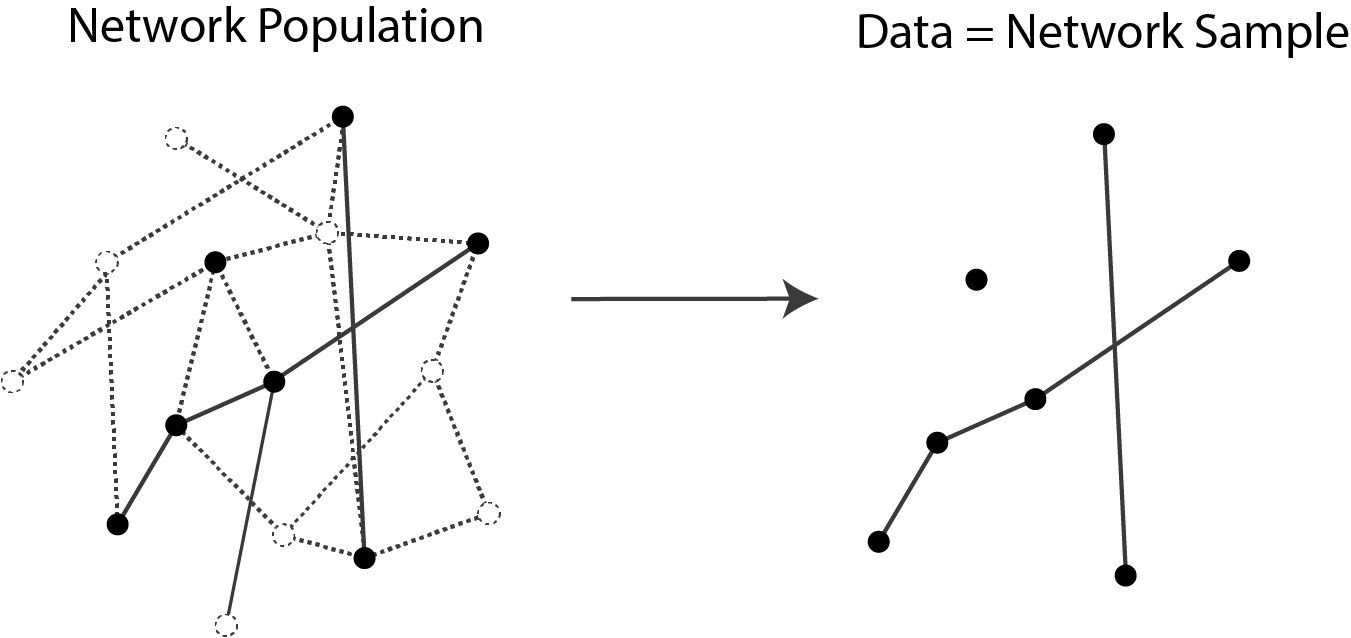
\includegraphics[width=0.8\linewidth]{foundations/ch1/Images/nodes.png}
    \caption[Only see subset of nodes]{The true underlying network has both solid and dashed edges and nodes, indicated in the left panel. However, when we sample the network on the right, our sample only includes the subset of nodes and edges that are solid.}
    \label{fig:ch1:nodes_ss}
\end{figure}


\subsubsection{We might only see a subset of the networks}

On a related note, let's put ourselves back in the mindset for the musician and non-musician brain networks from Example \ref{box:ch1:brainnet}. A team of psychologists might hypothesize that the brains of musicians tend to be much better connected in areas responsible for fine motor coordination and hearing, which are crucial skills for many instruments. To test this hypothesis, the psychologists could take one of two approaches. They could collect brain networks from every individual, or they could collect a subset of brain networks from groups of musicians and non-musicians in their area. In Figure \ref{fig:ch1:many_nets_ss}, we see an example where we only get to sample a subset of the networks in the underlying population. Despite the fact that the psychologists only studied a subset of musicians and non-musicians, with some statistical assumptions they can derive conclusions that will apply more broadly than just the group of people they analyzed.

\begin{figure}[h]
    \centering
    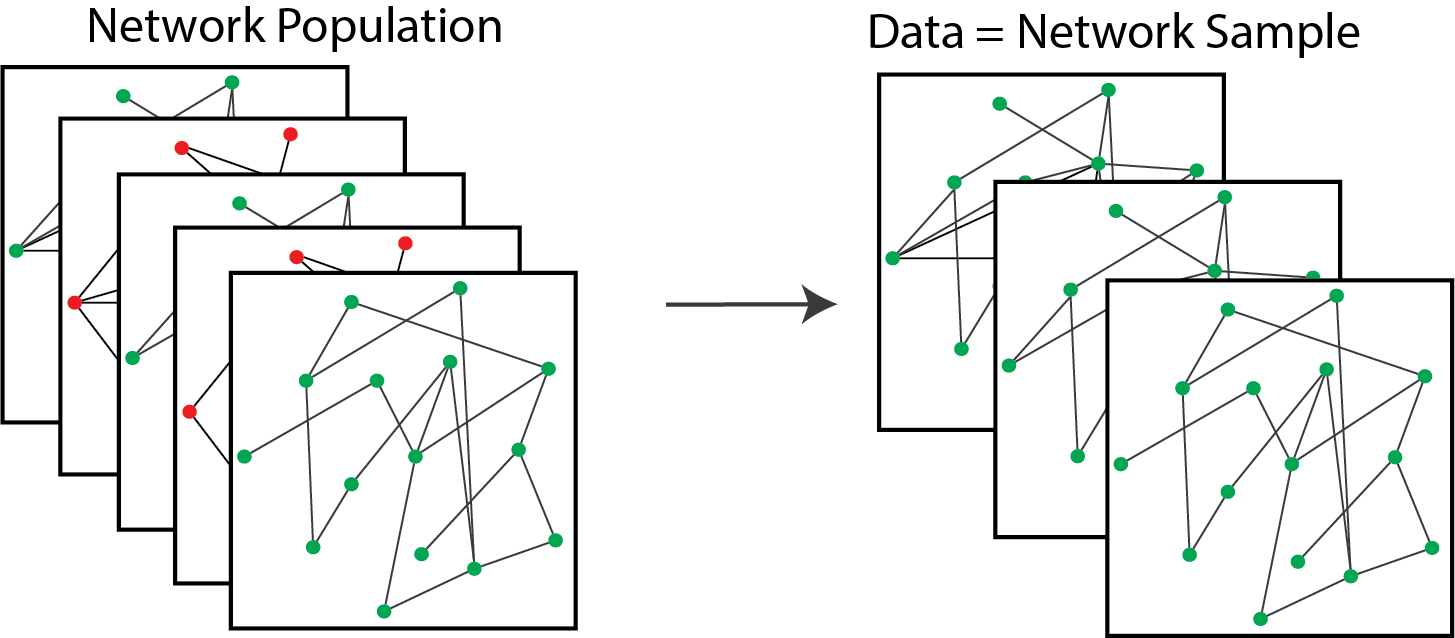
\includegraphics[width=0.7\linewidth]{foundations/ch1/Images/many_networks.png}
    \caption[Only see subset of networks]{The true underlying population contains many more networks than we are
able to actually sample. In the left panel, we have green and red
networks, but in the sample, we only get to see the green networks.}
    \label{fig:ch1:many_nets_ss}
\end{figure}

\subsubsection{Statistics allows us to bridge what we learn from what we see with what we didn't get to see}

In these cases, you have collected a \textit{sample}, which can be loosely defined as a subset of objects which is collected from the population in some way. The sample itself is where statistics comes into play. When you reach a conclusion, you do not want to reach a conclusion that only applies to the specific group of people, or the specific network, that you analyzed in your sample. Statistics allows you to be as specific as you can about how, exactly, conclusions that you reach on the sample apply to the general population. We summarize this idea in Figure \ref{fig:ch1:stat-learning}. Note that the network population may have a different interpretation depending on you specific network question, and might be populations of many networks, or populations of networks with some level of randomness or uncertainty as to how the network was obtained. Throughout this book, the sample itself, and how it relates to the underlying population, will always be in focus and should be at the forefront of your mind. 

\begin{figure}[h]
    \centering
    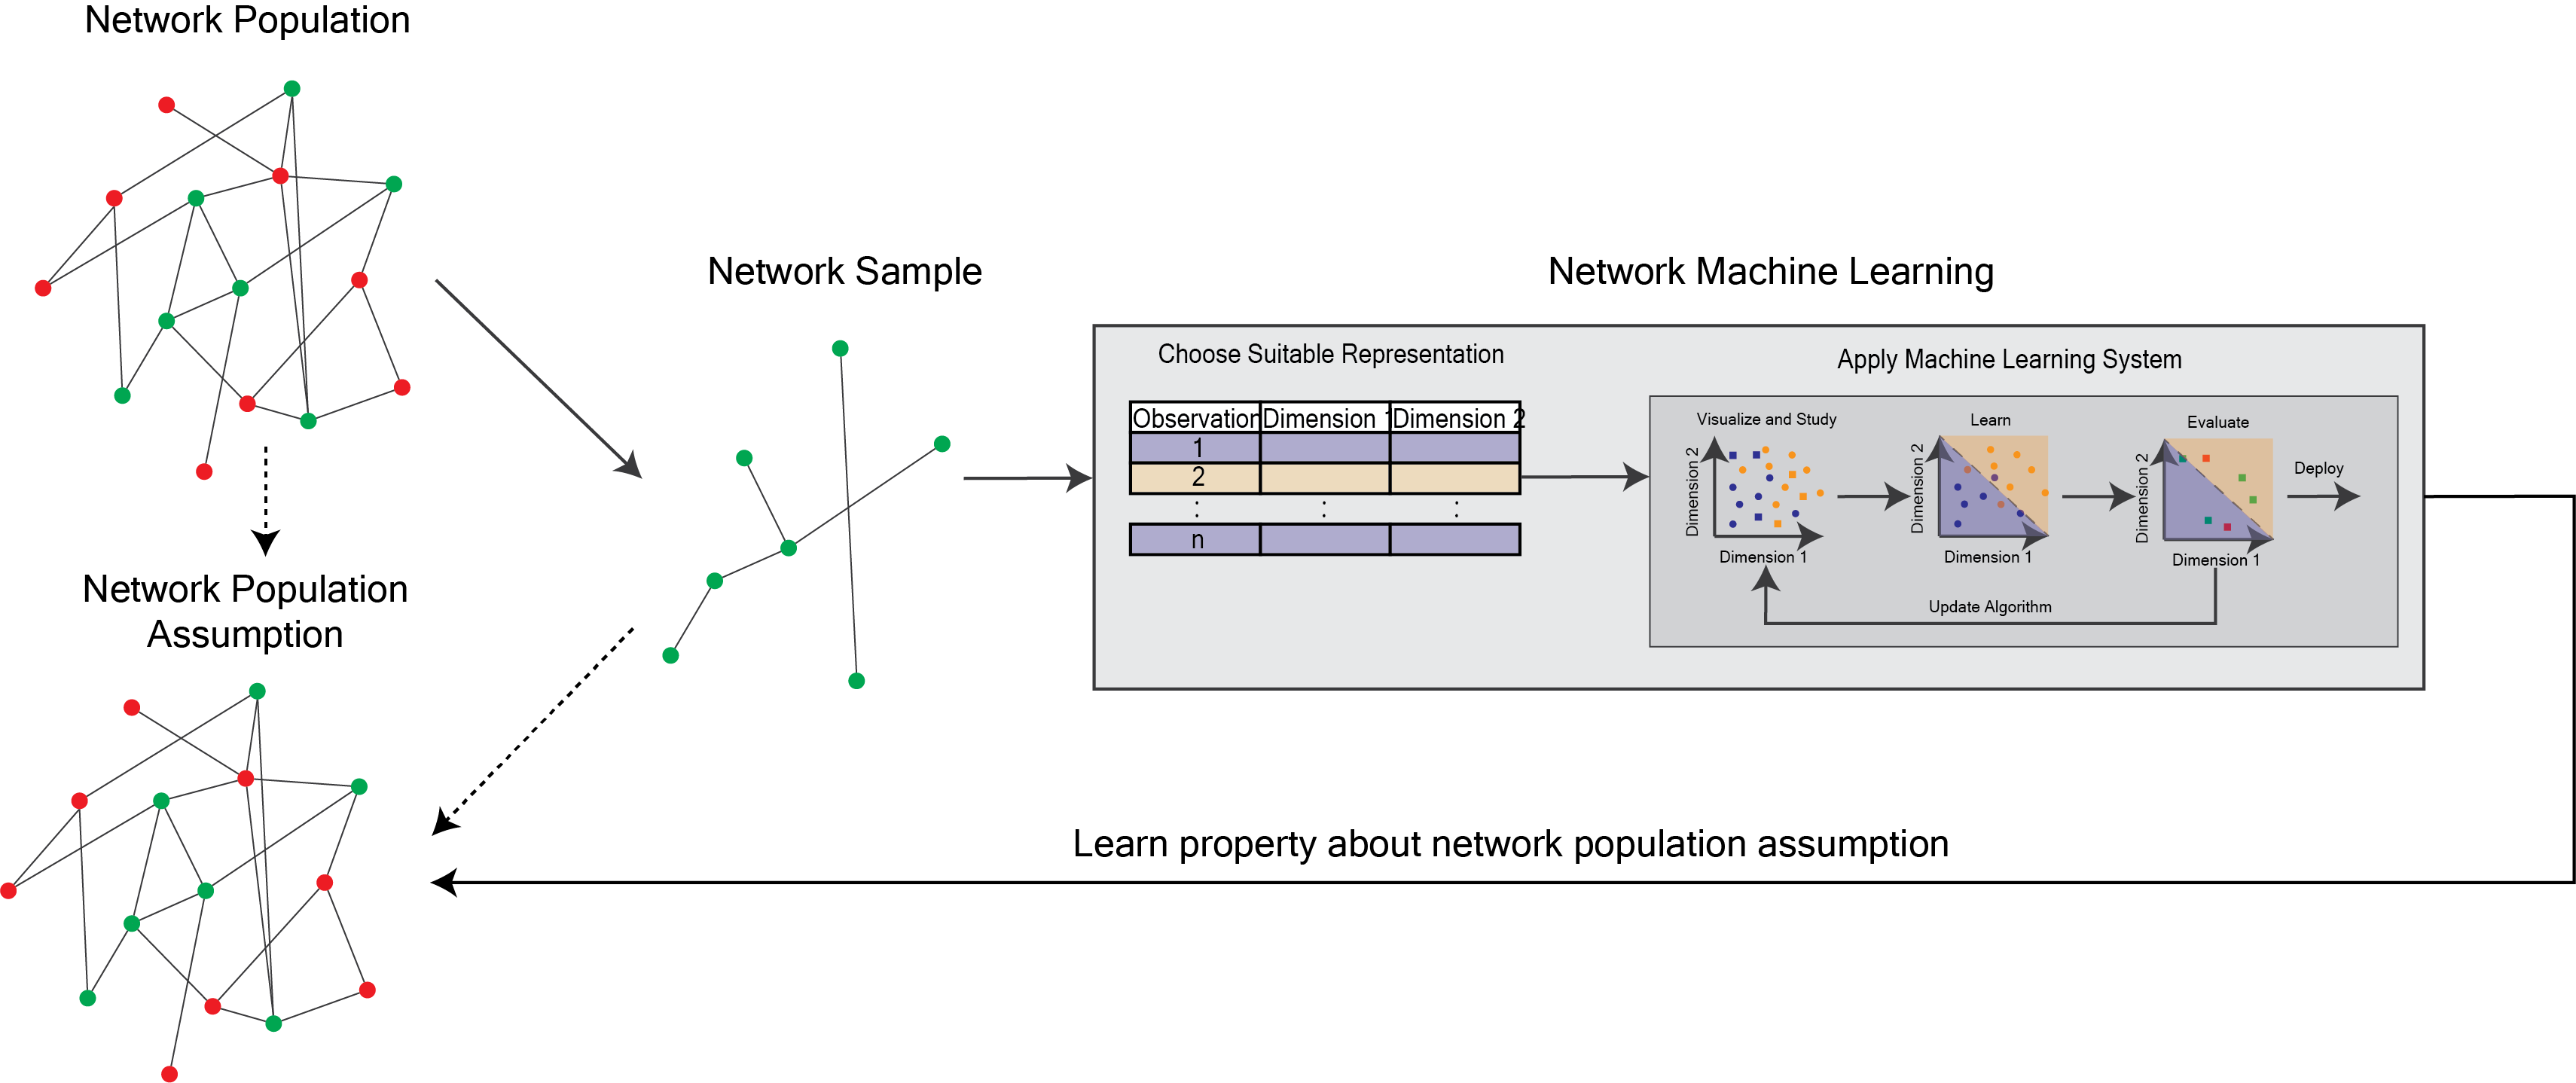
\includegraphics[width=\linewidth]{foundations/ch1/Images/apply.png}
    \caption[Statistical network machine learning]{We have a network population, which in this case, means a large network that we cannot properly observe. We obtain a sample of this network, and then use analyses on this sample and knowledge of how this sample was taken from the population to derive assumptions about our system. Ideally, this will faithfully represent the actual network population itself. Using network machine learning, we learn properties about the network population assumptions.}
    \label{fig:ch1:stat-learning}
\end{figure}


You {can} learn lots of valuable things about a sample without using statistics {at all}, and we will be sure to note when that is the case. However, if you want your conclusions to apply more broadly to the general population rather than the specific sample you collected, a reasonable way to do that quantitatively is using statistical learning.

\subsection{There are a variety of other challenges too!}

In Section \ref{sec:ch1:types}, you learned about some of the different types of network machine learning problems that we can start to address. Network machine learning is in its infancy, and these types of problems are constantly evolving. Deciding which group of categories your problem falls into, reshaping your question of interest to fit into problems that can be answered with existing techniques, the types of strategies that are at your disposal to answer your questions, or whether you need to develop new techniques all together to answer your question take lots of energy (and resources!). In the next few chapters, you'll see what example data analyses look like in network machine learning, which will hopefully give you a better idea of how these analyses are performed.

\newpage


\bibliographystyle{vancouver}
\bibliography{references}